\pdfoutput=1
\documentclass[11pt]{article}
\usepackage{ACL2023}
\usepackage{times}
\usepackage{latexsym}
\usepackage[T1]{fontenc}
\usepackage[utf8]{inputenc}
\usepackage{microtype}
\usepackage{inconsolata}
\usepackage{graphicx}
\usepackage{tabularx}
\usepackage{natbib}
\usepackage{multicol}
\setlength{\columnsep}{1cm}
\title{Improving Natural Language Inference with Contrastive Fine-tuning on ELECTRA Small}
\author{Stacy Roberts \\ EID: sr55278 \\robers23@utexas.edu}
\date{November 2024}

\begin{document}
\maketitle
\begin{abstract}
Natural Language models have used metrics such as test set accuracy to verify a model's performance in the real world. Utilizing test sets which are intimately tied to the training sets can lead to a high accuracy rating but not translate to similarly positive generalized performance. It has been found that models tend to find Data Artifacts in the body of training data, which are spurious connections between text that don't translate to generalized language well. The intent of this paper is to utilize contrastive datasets, designed not to alter the overall intent of the original corpus, to improve the ELECTRA small's understanding of underlying language and increase its accuracy on the contrastive set while not decreasing the accuracy of the original corpus.
\end{abstract}

\section{Introduction}
\subsection{Background}
Natural Language Inference (NLI) has become a popular task set for understanding how Language Models understand and interpret language. Models trained on a large corpus of data tend to perform well on test data built from the original training set, but do not perform as well when exposed to more complex language relationships. This is due to the fact that datasets typically have gaps in completeness which lead to corresponding gaps in a model's ability to understand language. NLI is a task set which categorizes the logical relationships between sentences.  It is used to test a system's ability to truly understand language. The tendency of a model is to rely on data artifacts inferred from the test data which are not based on actual premise/hypothesis inference, but on other spurious correlations. The NLI task attempts to clarify where a model is relying on these artifacts, allowing for focused training updates to improve a model's performance in real word testbeds. In this paper we utilize contrastive dataset augmentation to improve the Electra small model's accuracy on the Stanford NLI corpus.

\subsection{Motivation}

The chosen model, ELECTRA small, has the same architecture as BERT, but is smaller and more manageable on most modern systems making it accessible to researchers and developers without large compute power requirements. Given training is a computationally expensive endeavor, being able to utilize a smaller model allows more people access to Natural Language Processing. ELECTRA small is highly efficient even for its small size, achieving 89\% accuracy on the Stanford NLI corpus without utilizing any data augmentation or other techniques. This is due to the way it is initially trained. ELECTRA is a Replacement Token Detection (RTD) model. It is trained to distinguish "real" tokens from "fake" tokens generated by another network. This training method has allowed the model to perform rather well across different datasets.  The small version of ELECTRA has about a tenth of the parameters, a third of the hidden size and number of attention heads, although same number of layers as the regular size model. This makes it able to be trained on a single GPU in a few days to a higher accuracy than even the ChatGPT model which requires thirty times more compute power. \citealp{googleelectrablog}

In order to improve upon the baseline 89\% accuracy rating, we decided to utilize a contrast dataset approach. This approach takes premise/hypothesis pairs, makes a slight perturbation to the hypothesis which alters the label of the pair, expecting the initial accuracy to drop considerably.  The dataset is then utilized to further fine-tune the model, after which the model is evaluated on the original dataset as well as the contrast set to verify improvement. The intention is to remove the model's reliance on spurious data artifacts by pulling similar premise/hypothesis pairs closer together while simultaneously pushing dissimilar pairs further apart.  Contrast datasets are intended to clarify the transition boundaries on harder to separate data points, increasing a model's inference of natural language and therefore accuracy on real world testbeds. \citealp{localdecisionboundaries}

\subsection{Understanding Artifacts}

We fine tune trained our ELECTRA small discriminator model with the SNLI dataset, no other modifications to training code or data set initially.  Accuracy on this dataset was 89.7\%, as expected. However, it has been shown that datasets often have gaps in sentence patterns leading to models performing poorly in real world testbeds. In fact, testing done on this type of pre-trained model with just the hypothesis have shown that the model can achieve 67\% accuracy never having seen the premise.  It would seem counter-intuitive that a model could perform well predicting entailment without having a premise to entail to, but it is due to the artifacts of the training dataset that lead to this outcome.  \citealp{princeton} \citealp{premise4granted}

Analysis of the SNLI dataset leads to some interesting spurious correlations. Using Pointwise Mutual information (PMI) between word and entailment classification, it was found that there is a correlation between certain word tokens and the entailment of a hypothesis. Due to the nature of the SNLI corpus being descriptions of Flickr images, words such as animal, instrument, and outdoors showed up in entailed hypotheses more often, likely as more generic replacements for specific types of these elements. Similarly approximation words are used in place of specific numeric values (some, least, few), and explicit gender is removed to more generic human, person. Entailed hypothesis also tended to be shorter in nature, likely from removing words from the premise.

\begin{table}[h!]
    \centering
    \begin{tabularx}{0.45\textwidth} { 
  | >{\raggedright\arraybackslash}X 
  | >{\raggedright\arraybackslash}X | }
    \hline
    Premise & Hypothesis \\
    \hline\hline
        Black man singing with microphone & This is a singer \\
        \hline
        A person is folding laundry on the floor. & A man is folding his laundry while sitting on the floor \\
        \hline
    \end{tabularx}
    \caption{Entailment Word Replacement Biases}
    \label{tab:EWRB}
\end{table}

Neutral hypotheses are more likely to have modifiers and superlatives, likely in an attempt to add detail which may be plausible.  They are also more likely to have cause and purpose clauses, shown in the increase of words such as because in the subset.  

\begin{table}[h!]
    \centering
    \begin{tabularx}{0.45\textwidth} { 
  | >{\raggedright\arraybackslash}X 
  | >{\raggedright\arraybackslash}X | }
    \hline
    Premise & Hypothesis \\
    \hline\hline
        A man in his 30's is sitting on a curb of a busy sidewalk, dressed in a furry green costume. & The man just lost his job playing Oscar the Grouch at Sesame Place because he kicked a child. \\
        \hline
       People riding an old looking trolley & The trolley makes a rickety noise while moving \\
        \hline
    \end{tabularx}
    \caption{Neutral Word Replacement Biases}
    \label{tab:NWRB}
\end{table}
A strong indication of a contradictory hypothesis is the prevalence of negation words (nobody, no, not) along with the presence of words with the complete opposite meaning (naked for clothing or sleeping for a described activity). Even the length of the hypothesis can provide some artifacts. Long hypothesis tend toward a neural entailment prediction.  \citealp{princeton}

\begin{table}[h!]
    \centering
    \begin{tabularx}{0.45\textwidth} { 
  | >{\raggedright\arraybackslash}X 
  | >{\raggedright\arraybackslash}X | }
    \hline
    Premise & Hypothesis \\
    \hline\hline
        People crowded around toys on a table & People are eating \\
        \hline
       Two men holding their mouths open & Two men with gritted teeth \\
        \hline
    \end{tabularx}
    \caption{Contradiction Word Replacement Biases}
    \label{tab:CWRB}
\end{table}
The figure below shows the probability word mass of each class within the SNLI corpus. Note that the entailed class has the highest probability of less than 7 word tokens on average per hypothesis, while neutral has the widest distribution skewed towards the highest number of tokens of any of the classifications.
\begin{figure}[h!]
    \centering
    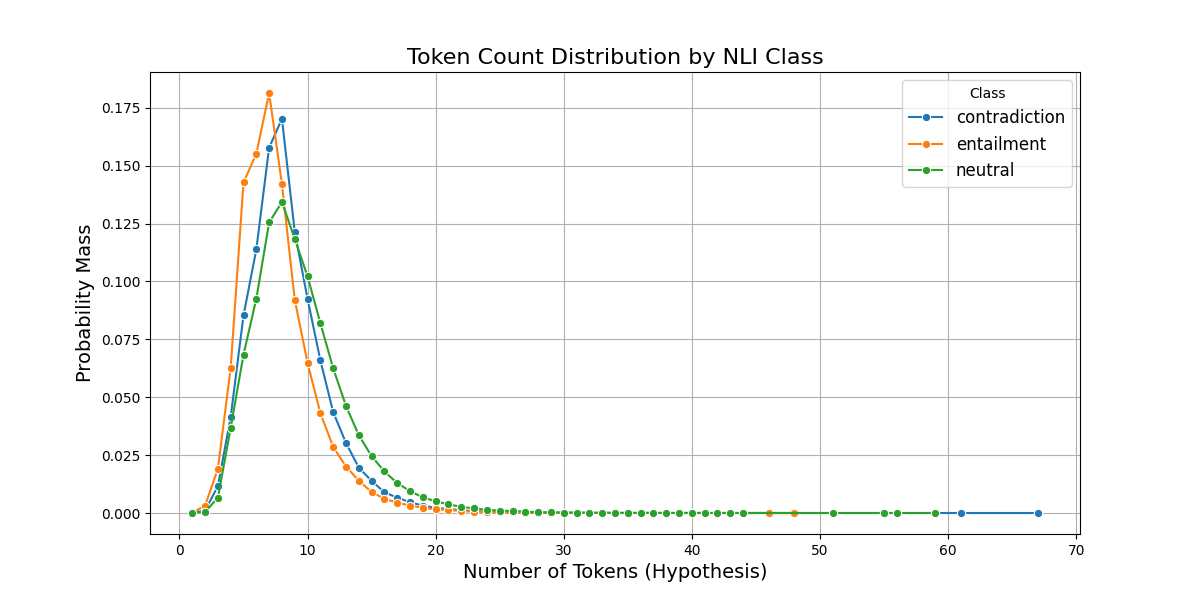
\includegraphics[width=1.0\linewidth]{Figure_tokenvsprobmass.png}
    \caption{Probability Mass Function of Hypothesis Length by Class, SNLI}
    \label{fig:}
\end{figure}

\section{Related Works}
Natural Language Inference:
Review NLI datasets like SNLI, MultiNLI, and other benchmarks.
Discuss existing approaches (e.g., BERT, RoBERTa, and ELECTRA).

Note that Data Artifacts are from the training corpus. The model learns that majority of long hypotheses tend to be neutral, doesn't check the premise to guess this pretty well. Certain words are more prevalent in entailed or contradictory hypotheses, causing the model to skew the classification based solely on word choice of hypothesis.  (all in googleelectrablog)

Contrastive Learning in NLP:
Initial fine-tune training of our Electra small model was performed on the Stanford Natural Language Inference (SNLI) Corpus dataset. This dataset consists of around 570k premise/hypothesis pairs. \citealp{snlicorpus}

Ran on SNLI dataset. Achieved 89.7\% accuracy without any changes
Approach was to work with Contrastive sets in an attempt to push similar premise/hypothesis pairs closer together and contradictory pairs further apart. This should increase the model's ability to correctly predict entailment of these difficult boundary cases.

Provide a brief overview of contrastive learning methods and their applications in semantic understanding.
Cite recent works leveraging contrastive learning for improving NLI or related tasks.
Smaller Language Models:
Discuss the importance of small models for resource-constrained settings.
Highlight the trade-offs between model size, accuracy, and generalization.

\section{Model}
\subsection{Pre-trained Model}

We began with a pre-trained Electra Small Discriminator model from HuggingFace. For the NLI (Natural Language Inference) task, the ElectraForSequenceClassification head was selected as the fine tuning head. 

explain what the small electra is.
Initially trained on either snli dataset (570k elements) for 3 epochs. Achieved 89.7\% accuracy on the evaluation set. Found low confidence on errors but skewed to neutral.
\subsection{Evaluation Trials}
Retrained on a very small subset (10k) for 5 epochs not realizing how big the dataset was, then immediately retrained again on half the dataset (275k) for 5 epochs. Now my accuracy on eval was 88.6\% but the data analysis showed more skew towards irrelevant.

Retrained on entire dataset for 5 epochs and am finding higher confidence on wrong predictions now. Longer wasn't better.

\section{Analysis of errors}
\subsection{Hypothesis-Premise SNLI}

Stored incorrect predictions into a jsonl file for analysis. Used mathplotlib and other libraries to work on model.
What analysis did I do on the outputs? Can i get dataset cartography to work?

All incorrect predictions came with super low confidence. Nothing higher than 40\% when trained only 3 epochs. When trained 5 epochs it went up significantly to nearly 50\% on some of the outputs.

there seems to be a length issue. If the premise is long and the hypothesis entailed in the early half of the sentence, model often predicts neutral.

Incorrect labels skewed more to neutral, entailment and irrelevant were both lower than gold label standard totals.

Seeing some premises that are long with the hypothesis clearly supported/entailed by the later half of the sentence. 

Some pairs require some inference (they were throwing tomatoes at each other - they were having a food fight)

Trained a single epoch on a glue:mnli dataset and accuracy dropped to 71.8\%  but after the refresh on snli and contrastive set this dropped to 69\%

Don't forget to add the chart on length of premise and length of hypothesis of the incorrect predictions

Ran small contrastive dataset in eval mode. Model only achieved 44\% accuracy.

\subsection{Contrast Sets}
The incorrectly predicted premise/hypothesis pairs from training were stored in a file, along with the logits produced by the model for each entailment, neutral, and contradictory, and both the gold and predicted labels. The logits were converted to probabilities using a softmax. Next the confidence of the model in its prediction was calculated. Model confidence is a useful metric to explore where the model is relying on data artifacts over language inference. A low confidence is generally easier to perturb and move the model to correctly identify classification than a high confidence mis-prediction. 

Using the confidence score, we built a small contrast dataset by hand, minorly perturbing the hypothesis to alter the label of the premise/hypothesis pair on the pairs with high confidence.   

Created pairs of premise/hypothesis sets where one was the original and the other changed a word or some small phrasing to change the label. Evaluated the model on these pairs. Accuracy dropped to 44\%  Provide examples here

\section{Experiments}
\subsection{SNLI}

Describe the SNLI dataset (it is balanced) \citealp{dataAug}

\subsection{Contrastive DataSets}

Cosine similarity used generally to build a contrastive dataset. Intention is to pull similar pairs (entailment) closer together and push opposite pairs (contradictive) further apart.

Contrastive sets are for evaluation to pinpoint weaknesses in the model learning. Have to use this info to figure out how to fix the model.

Data augmentation with this contrastive set used to fine-tune the model.
Add chart that shows accuracy with snli vs accuracy with contrast set (two bars just 89.7\% and 44.5\%)

I'm looking for increased accuracy on the contrast set after the retraining.

Took an snli trained (5 epochs, full dataset), trained on a small contrast dataset (61 elements from original failed predictions).  Achieved a 78\% accuracy on snli, but increased the output of the contrast set to 72.6\%

retrain on 10k samples of snli accuracy on snli is: 89.8\%
retrain on contrast\_data.jsonl with lr of 1e-6, eval on snli: 89.87\%  contrast: 77.4

Added to contrast set with small confidence pairs. Retrained on contrast set, then on snli subset to refresh. SNLI accuracy now at 89.1\% 49 on contrast
After retrain on contrast, contrast at 79.3 snli at 89.4\%

\section{Conclusion}

\bibliographystyle{apalike}
\bibliography{references}
%\end{multicols*}

\end{document}